\chapter{Counting Circle Tangencies\label{chap:circle}}

Here we shall discuss the problem of counting the number of tangencies in a suitably non-degenerate collection of circles. We say two circles are tangent if their intersection contains a single point.
The set of unordered pairs of circles in a collection $\CE$ which are mutually tangent are called the tangencies of the collection and is denoted $\tau(\CE)$. 
\section{Trivial Bounds}
\begin{theorem}[Trivial Bound] \label{thm:trivial-circle-bound}
    Let $\CE$ be an arbitrary finite collection of circles. Then the number of tangencies $|\tau(\CE)|$ is bounded as follows:
    \[
        |\tau(\CE)| \leq |\CE|^2.
    \] 
\end{theorem}
Stated for arbitrary collections of circles the problem is not particularly interesting as the above bound turns out to be asymptotically tight. 
\begin{example}
Denote a circle centred at $(x,y)$ with radius $r$ as $\gamma (x,y,r)$.
Consider the following collection of $N+1$ circles:
\begin{align*}
    C_0 &= \gamma\left(0,0,1\right) \\
    C_1 &= \gamma\left(\frac{1}{2},0,\frac{1}{2}\right) \\
    C_2 &= \gamma\left(\frac{3}{4},0, \frac{1}{4}\right) \\
    &\vdots \\
    C_N &= \gamma\left(1- \frac{1}{2^N}, 0, \frac{1}{2^N}\right)
\end{align*}
Each circle in our collection $\CE = \{ C_i \ | \ 0 \leq i \leq N\}$ is tangent to $N$ other circles at the point (1,0). 
Hence $|\tau(\CE)| \sim N^2 \sim |\CE|^2$. 
\begin{figure}[h]
    \centering 
    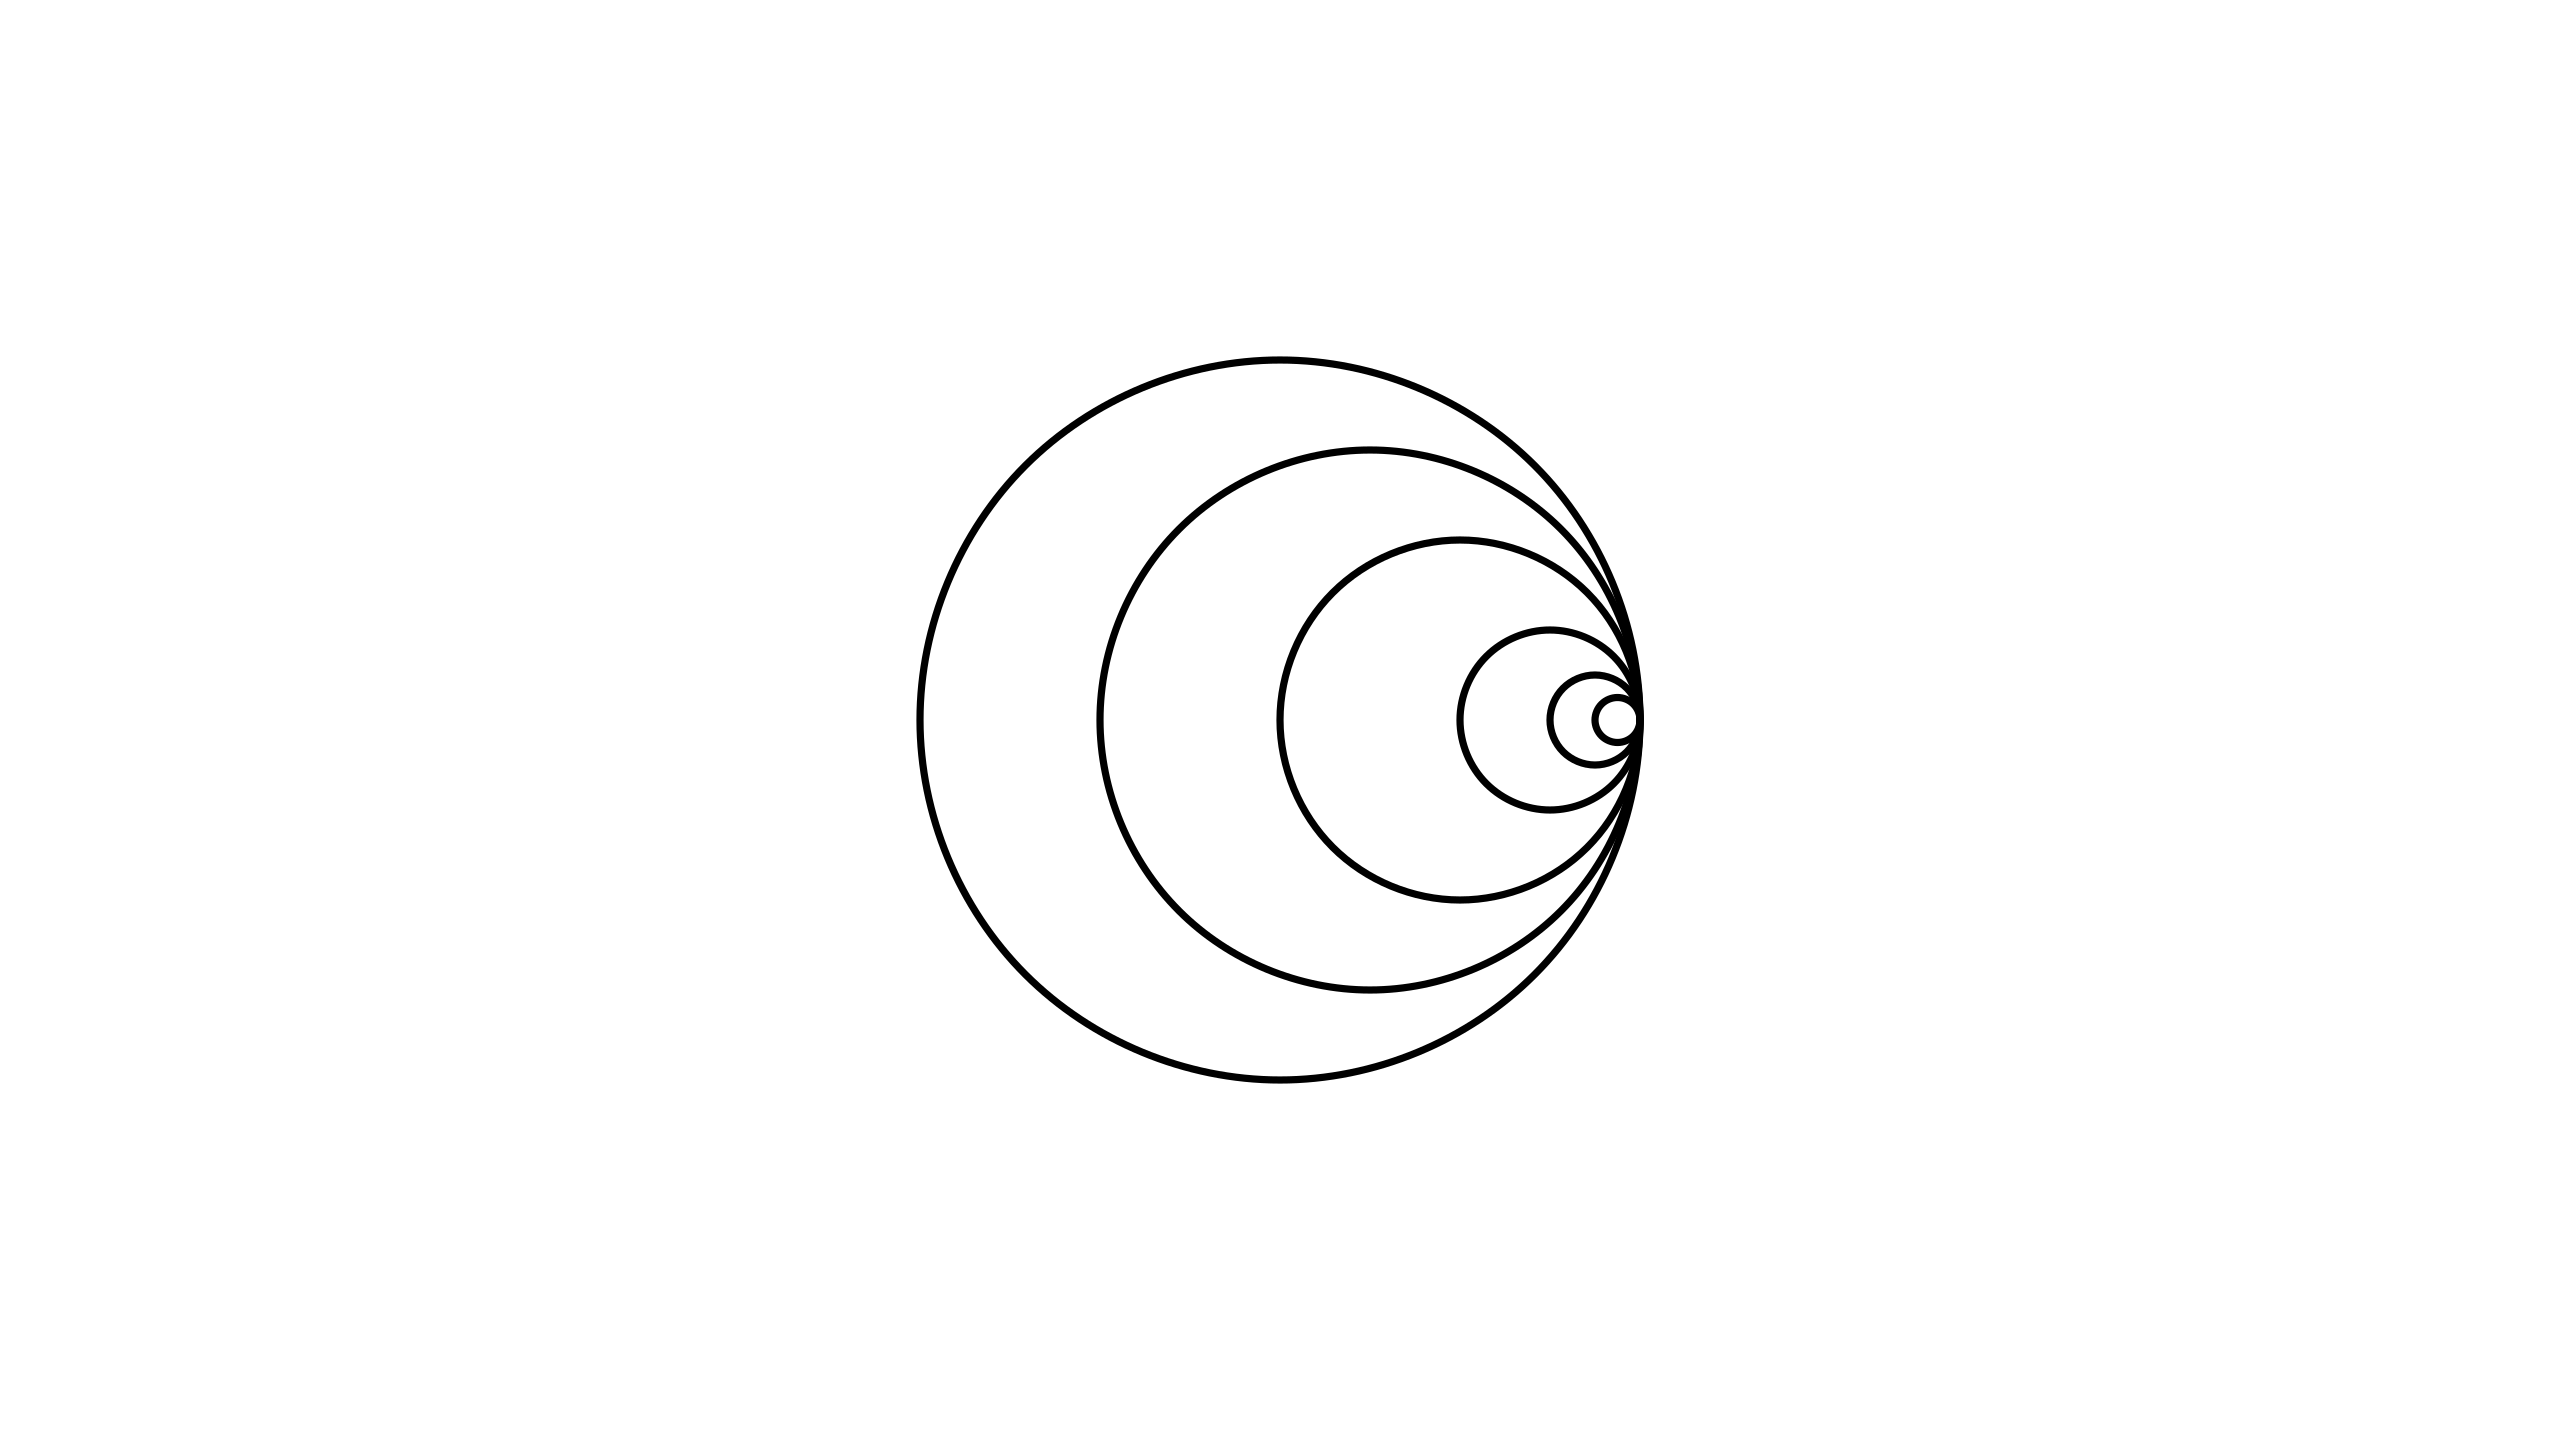
\includegraphics[width=0.8\textwidth]{images/circles_degen_case_ManimCE_v0.15.1.png}
    \caption{A collection of circles in $\RR^2$ with $N^2$ tangencies.}
    \end{figure}
\end{example}

Instead we shall look at collections of circles that satisfy a single non-degeneracy condition. We consider collections of circles 
such that no three are mutually tangent at a common point. The best known examples leverage our asymptotically tight \hyperref[thm:S-T]{Szemerédi-Trotter Theorem} examples:
\begin{example}
    Let $\ES$, $\LL$ be collections of $N$ points and $N$ lines respectively such that the \hyperref[thm:S-T]{Szemerédi-Trotter Theorem}'s bound is asymptotically tight. 
    In particular, they determine $\sim N^{4/3}$ point-line incidences. 
    Let $C_1$ denote the collection of unit circles centred at the points of $\ES$. 
    Let $C_2$ denote the collection of lines obtained by translating each line $\ell in \LL$ one unit in the $\ell^{\perp}$ direction.
    If $(p,\ell) \in \ES \times \LL$ is a point-line incidence from our original collection, then the corresponding circle-line pair will be tangent.
    Performing an inversion transform about a point that does not lie in any of the circles or lines, our collection $\CE = C_1 \cup C_2$ becomes a 
    collection of $2N$ circles that determine $N^{4/3}$ tangencies. \label{ex:circle-lower-bound}
 \end{example}

We shall now present a bound from a recent paper of Ellenberg-Solymosi-Zahl which uses the polynomial method.\cite{ellenberg2016new}

\begin{theorem}
    Given a finite collection $\CE$ of $N$ circles in the plane such that no three are tangent at a common point, 
    then the number of tangencies $|\tau(\CE)|$ obeys:   \label{thm:circle-tangencies}
    \[
        |\tau(\CE)| \lesssim N^{3/2}
    \]
\end{theorem}

It is not obvious how to apply the polynomial method in the current formulation. 
We will perform a lifting  of our circles into algebraic curves $\RR^3$, 
preserving tangencies between circles in the plane as intersections between their lifted curves in $\RR^3$. 
This transforms the problem from a tangency problem to an incidence problem, and reduces the required degree of polynomial needed to interpolate.
In general Lemma \ref{lem:paramcounting} tells us that if we are to interpolate a set of $M$ points in $\RR^d$ by a polynomial $P$, then the degree of $P$ is $O(M^{1/d})$, 
so increasing the dimension of the problem yields a more controlled degree of the polynomial required.

\section{Lifting of circles to $\RR^3$}

We shall now discuss this lifting in detail. Let $\gamma \subset \RR^2$ be a circle in the plane of radius $r_{\gamma}$ centred at $(x_\gamma, y_\gamma)$. 
We define the lifting transform of the circle as: \[
    \beta(\gamma) = \left \{ (x,y,z) \in \RR^3 \ \big | \ (x-x_\gamma)^2 + (y-y_\gamma)^2 = r_\gamma^2, \ z = - \frac{x-x_\gamma}{y-y_\gamma} \right \}.
\]  
Clearly $\beta(\gamma)$ is an algebraic curve, so now we shall examine the correspondence between mutually tangent circles. Notice that $z$ is defined as the reciprocal of the slope of the tangent line
at the point $(x,y) \in \gamma$.

\begin{lemma}
    Let $\beta$ be the transform defined as above. 
    Then two circles $\gamma, \gamma' \subset \RR^2$ are tangent if and only if $\beta(\gamma) \cap \beta(\gamma') \neq \emptyset$.    \label{lem:beta-lift}
\end{lemma}
\begin{proof}
If $\gamma$ and $\gamma'$ are tangent then there exists a point $(x,y) \in \gamma \cap \gamma'$ and
at a point of tangency we have that the slopes of the tangent lines coincide for $\gamma$ and $\gamma'$. Explicitly $\frac{x-x_\gamma'}{y - y_\gamma'}= \frac{x-x_\gamma}{y - y_\gamma} = z$.
Hence $(x,y,z) \in \beta(\gamma) \cap \beta(\gamma')$ and thus $ \beta(\gamma) \cap \beta(\gamma') \neq \emptyset$.

In the other direction, assume there exists some $(x,y,z) \in \beta(\gamma) \cap \beta(\gamma')$. 
Clearly $(x,y) \in \gamma \cap \gamma'$ and the slopes of the tangent lines at this point are equal,
hence we conclude $\gamma$ is tangent to $\gamma'$.
\end{proof}
This one-to-one correspondence between tangencies in $\RR^2$ and incidences in $\RR^3$ is the key idea behind the proof. 
For those more algebraically inclined, what we are doing here is equivalent to looking at the tangent bundles of our circle in the projective space, hence we 
are preserving intersections.

We will need a Bezout-type result which bounds the number of intersections between curves with no common components.
\begin{lemma}[Bezout's Theorem for Plane Algebraic Curves]     \label{lem:Bezout}
   Let $Z_1$ and $Z_2$ be the zero sets of two polynomials over $\RR[X,Y]$ and suppose $\deg Z_1 > \deg Z_2$. Then one of the following holds:
   \begin{align*}
    |Z_1 \cap Z_2 | &\leq \deg Z_1 \deg Z_2 \\
    \text{ or } &Z_2 \subset Z_1
   \end{align*}
\end{lemma}


\section[Ellenberg-Solymosi-Zahl's Proof]{Ellenberg-Solymosi-Zahl's Proof of Theorem \ref{thm:circle-tangencies}}
In this proof, we will need to ensure our tangencies
are sufficiently uniformly distributed among our circles. We can refine our collection such that this is the case by the following lemma.

\begin{lemma}[Uniform Refinement]
    Let $\CE$ be a collection of $N$ circles and suppose that $|\tau(\CE)| \gtrsim N^{\alpha}$. 
    Then we can refine our collection to a collection $\CE' \subset \CE$ such that every circle in $\CE'$ is mutually tangent to $\gtrsim N^{\alpha -1}$ other circles in $\CE'$, $|\tau(\CE')| \gtrsim N^{\alpha}$, and $|\CE'| \gtrsim N^{\alpha/2}$. \label{lem:uniform-refine}
\end{lemma}

\begin{proof}
We proceed by a stopping time argument.
Let $\tau(\CE)$ be the set of tangencies of the circles in $\CE$. Let $\CE_0 = \CE$ and let $c_1$ be a fixed constant to be chosen later. If there exists a circle $\gamma \in \CE_0$ such that $|\{ \gamma' \ |\ (\gamma, \gamma') \in \tau(\CE_0)\}| < c_1 N^{1/2}$
remove it from the collection and label the new refined collection as $\CE_1$. From this refined collection, if there exists a circle $\gamma$ such that $|\{\gamma'\ |\ (\gamma, \gamma') \in \tau(\CE_1)\}| < c_1 N^{1/2}$ we remove it and label the remaining collection as $\CE_2$.

After repeating this process $M$ times until there are no more circles $\gamma$ that satisfy $|\{\gamma'\ |\ (\gamma, \gamma') \in \tau(\CE_M)\}| < c_1 N^{1/2}$, at each step removing a circle that contributes only a small number of tangencies, we attain a collection $\CE_M$.
 We claim that $|\tau(\CE_M)| \gtrsim N^{\alpha}$, and that $|\CE_M| \gtrsim N^{\alpha/2}$.

For the first claim, observe that at each step $i$ we are reducing $\tau(\CE_i)$ by at most $c_1 N^{\alpha -1}$.  Thus,
\begin{align*}
    |\tau(\CE_M)| &\geq |\tau(\CE_0)| - M c_1 N^{\alpha -1} \\
    &> c_0 N^{\alpha} -  M c_1 N^{\alpha -1} \\ 
    &> c_0 N^{\alpha} - c_1 N^{\alpha} \\
    |\tau(\CE_M)| &> \frac{c_0}{2} N^{\alpha}. \qquad (\text{by choosing } c_1 = c_0/2 )
\end{align*}
We now provide a lower bound on the cardinality of our refined set $\CE_M$. We have the trivial inequality $|\tau(\CE_M)| \leq |\CE_M|^{2}$. 
Combining this with the result above, we attain $|\CE_M| \gtrsim |N|^{\alpha/2}$.
\end{proof}
In a similar fashion to our arguments in the Kakeya\todo{write coherent sentence} problem we will be arguing by contradiction, however here we will be arguing that if the zero set of a polynomial contains too many of a certain first type of object, 
it must contain many more of a second kind of object. 




We can now prove the main theorem. 
\begin{proof}[Proof of Theorem \ref{thm:circle-tangencies}]
    Given an arbitrary collection of circles $\CE$ with $\gtrsim N^{3/2}$ tangencies, Lemma \ref{lem:uniform-refine} with $\alpha = \frac{3}{2}$ 
    allows us to reduce to a collection
     $\Gamma$ where each circle is tangent to  $\gtrsim N^{1/2}$ other circles using the previous lemma. 
    After applying a small rotation, we can assume that the tangent line at each point of tangency does not point vertically in the $y$-direction.
    Let $\beta (\Gamma) = \{ \beta(\gamma) : \gamma \in \Gamma \}$, where $\beta$ is the lifting transform defined earlier,
    Recall from Lemma \ref{lem:beta-lift} that two circles $\gamma_1$ and $\gamma_2$ are tangent if and only if $\beta(\gamma_1) \cap \beta(\gamma_2) \neq \emptyset$.

    Suppose $(x,y,z) \in \beta(\gamma_1) \cap \beta(\gamma_2) $ for some $\gamma_1 \neq \gamma_2$. 
    Then $$(0,0,1) \in \text{span} \left( T_{(x,y,z) }\beta (\gamma_1), T_{(x,y,z) }\beta (\gamma_2)\right).$$
    In other words, at the intersection of $\beta(\gamma_1)$ and $\beta(\gamma_2)$ their tangent vectors span a vertical subspace of $\RR^3$. 
    We can establish this by examining a parameterisation of $\gamma_1$ and $\gamma_2$ in the neighbourhood of $(x,y)$.
    Define $f_i (t), \ i \in \{1,2\}$ such that $(t+x, f_i(t))$ is a parameterisation of $\gamma_i$ in the neighbourhood of $(x,y)$ for all $t$ in a small neighbourhood of 0. In particular $f_i(0) = y$. Taking the first derivative and evaluating at $t=0$:
    \[
        \frac{df_i}{dt}(0) = -\frac{x- x_{\gamma_i}}{y- y_{\gamma_i}}
    \]
    Since $\gamma_1$ is tangent to $\gamma_2$ at $(x,y)$ the slopes of their tangent lines coincide at that point so $\frac{df_1}{dt}(0) = \frac{df_2}{dt}(0)$. Now taking the second derivative and evaluating at $t=0$:
    \[
        \frac{d^2f_i}{dt^2}(0) = -\frac{(y- y_{\gamma_i})^2 + (x- x_{\gamma_i})^2}{(y- y_{\gamma_i})^3} = -\frac{r^2_{\gamma_i}}{(y- y_{\gamma_i})^3} 
    \]
    Since $\gamma_1$ and $\gamma_2$ are distinct quadratic curves, $\frac{d^2f_1}{dt^2}(0) \neq \frac{d^2f_2}{dt^2}(0)$. 



    In the neighbourhood of $(x,y,z)$, $\beta(\gamma_i)$ is parametrised by $\left(t,f_i (t) ,\frac{df_1}{dt}(t) \right)$ as the slope of the tangent to the circle is given by $\frac{df_1}{dt}(t)$.
     It follows that the tangent vector
    $\left(1,\frac{df_i}{dt}(0), \frac{d^2f_i}{dt^2} (0) \right)$ generates the vertical space $T_{(x,y,z)} \beta(\gamma_i)$. Thus 
    \begin{align*} (0,0,1) &\in \text{span}\left( \left(1,\frac{df_1}{dt}(0), \frac{d^2f_1}{dt^2} (0) \right) - \left(1,\frac{df_2}{dt}(0), \frac{d^2f_2}{dt^2} (0) \right) \right)
    \\ &\subset \text{span} \left( T_{(x,y,z) }\beta (\gamma_1), T_{(x,y,z) }\beta (\gamma_2)\right). 
    \end{align*}

    We will now interpolate all points of intersection with a minimal polynomial of suitably low degree, and show that if this contains too many intersections it must also contain the curves. 
    Then due to the tangent vector spanning the $z$-axis we will be able to achieve a contradiction.

    Let $P \in \RR[x,y,z]$ be a non-zero polynomial of minimal degree that vanishes on all intersections between the curves in $\beta (\Gamma)$. 
    This polynomial interpolates $\sim N^{3/2}$ points in $\RR^3$, so by Lemma \ref{lem:paramcounting}
    the degree of $P$ is $\lesssim \left(N^{3/2}\right)^{\frac{1}{3}} =  N^{1/2}$. 

    Due to our refinement each $\gamma \in \Gamma$ is 
    tangent to $\gtrsim N^{1/2}$ circles and each of these tangencies occur at a distinct point by our non-degeneracy condition.   
    Hence we have that $P$ vanishes at $\gtrsim N^{1/2}$ points on each curve in $\beta (\Gamma)$.
    By \hyperref[lem:Bezout]{Bézout's theorem} we have that $P$ vanishes on all curves in $\beta(\Gamma)$ as:
    \[
    \deg (P) \deg (\beta(\gamma))  \lesssim \# \{ P \cap \beta(\gamma)\}  
    \]
    for suitable choice of constants. 

    By our result above, if $(x,y,z)$ is a point where two curves from $\beta (\Gamma)$ intersect, then $\partial_z P (x,y,z)  =0 $. 
    Thus by the same Bezout argument $\partial_z P$ is also a polynomial which vanishes on all curves in $\beta(\Gamma)$. 

    Since $P$ was a non-zero polynomial of minimal degree that vanishes on all the curves in $\beta (\Gamma)$, we must conclude 
    $\partial_z P \equiv$ 0. By the minimality if $P$ we must have that $P(x,y,z) = Q(x,y)$ for some $Q \in \RR[x,y]$ with degree $\lesssim N^{1/2}$. 
    But this implies that there must be at least of the $N^{3/4}$ circles in our original collection must also be contained in $Z(Q)$.
    This is a contradiction, as $Q$ has degree $\sim N^{1/2}$ whereas $\cup \gamma$ has degree $2N^{3/4}$.
    Thus $\beta(\Gamma)$ has $\lesssim N^{3/2}$ curve-curve incidences, so we can conclude that $\Gamma$ has $\lesssim N^{3/2}$ tangencies.
\end{proof}

\section[New Proof via Polynomial Partitioning]{A New Proof via Polynomial Partitioning for Varieties}
In this section we shall present a new proof of Theorem \ref{thm:circle-tangencies}. 
There are a few key differences between both methods of proof. In the following proof, 
it is no longer required to ensure the uniform distribution of tangent points among each circle in our collection, so we will not
have to use Lemma \ref{lem:uniform-refine}.
Secondly, we will partition $\RR^3$ using a polynomial of controlled degree and leverage our \hyperref[thm:trivial-circle-bound]{trivial bound} in each cell.
Slight care will be needed to deal with intersections of curves in the zero set, which we do via a recursive style argument.

We begin by introducing the main tool for this proof, 
an extension of the \hyperref[thm:PolyPartioning]{polynomial partitioning} theorem to algebraic varieties instead of just points (which are in some sense 0-dimensional varieties). 

\begin{lemma}[Polynomial Partitioning for Algebraic Varieties]
    Suppose $\Gamma$ is a set of $k$-dimensional varieties in $\RR^n$. For any positive integer $D$ there exists a non-zero polynomial $P$ of degree at
    most $D$ such that each connected component of $\RR^n \backslash Z(P)$ intersects $\lesssim D^{k-n} |\Gamma|$ varieties $\gamma \in \Gamma$.
    \label{lem:poly-part-var}
\end{lemma}
We shall not prove this here. A proof of this can be found as Theorem 0.3 in the original paper of Guth presenting the result.\cite{guth2015polypartvar}
\todo{add sketch of proof?}

\begin{proof}[Proof of Theorem \ref{thm:circle-tangencies} by Polynomial Partitioning]
Relabel $\CE$ as $\Gamma$ for convenience. Again, we perform the lifting transform $\beta$ on each $\gamma \in \Gamma$. 
We have a collection of $N$ 1-dimensional varieties in $\RR^3$ upon which we shall use our \hyperref[lem:poly-part-var]{polynomial partitioning} lemma
to find a polynomial $P$ such that each cell of $\RR^n \backslash Z(P)$ intersects $\lesssim N D^{-2}$ varieties. 
$\RR^3 \backslash Z(P)$ partitions the space into $\sim D^3$ cells. 
Let us label the interior of each of these cells as $\{\Omega_i \ | \ 0 \leq i \lesssim D^3 \}$, and further label the set of varieties in $\Gamma$ that pass through a given cell $\Omega_i$ as $\Gamma_i$.

We can now define the following complimentary sets based on whether the variety is contained entirely in $Z(P)$:
\begin{align*}
    C_1 &= \{ \beta(\gamma) \ |\ \beta(\gamma \not \subset Z(P) \}\\
    C_2 &= \{ \beta(\gamma) \ |\ \beta(\gamma)  \subset Z(P) \}
\end{align*}
Notice here that $\beta(\Gamma) = C_1 \cup C_2$. Recalling the correspondence between incidences between our curves and tangencies of the circles, we define the following
incidence sets and hence have the following expression for $|\tau(\Gamma)|$:
\begin{align*}
    I(C_1, C_1) &= \{(\beta(\gamma), \beta(\gamma')) \ |  \ \beta(\gamma), \beta(\gamma') \in C_1, \ \beta(\gamma) \cap \beta(\gamma') \neq \emptyset \} \\
    I(C_1, C_2) &= \{(\beta(\gamma), \beta(\gamma')) \ |  \ \beta(\gamma)\in C_1, \beta(\gamma') \in C_2, \ \beta(\gamma) \cap \beta(\gamma') \neq \emptyset \} \\
    I(C_2, C_2) &= \{(\beta(\gamma), \beta(\gamma')) \ |  \ \beta(\gamma), \beta(\gamma') \in C_2, \ \beta(\gamma) \cap \beta(\gamma') \neq \emptyset \} \\
    |\tau(\Gamma)| &= |I(C_1, C_1)| + |I(C_1, C_2)| + |I(C_2, C_2)|.
\end{align*}
We now proceed by calculating the cardinality each of these sets. The case for $I(C_1,C_1)$ will use our \hyperref[thm:trivial-circle-bound]{trivial bound} and bezout's
theorem. Calculating for $I(C_1,C_2)$ is again straightforward by Bezout. 
The interesting case here is $I(C_2,C_2)$, where we will be forced to argue via a recursive style of argument.

We begin with the intersections that occur between varieties not entirely contained in the zero set:
\begin{align*}
    I(C_1,C_1) = &\{ (\beta(\gamma), \beta(\gamma')) \ |  \ \beta(\gamma), \beta(\gamma') \in C_1, \ \beta(\gamma) \cap \beta(\gamma') \in \RR^3 \backslash Z(P)\} \\
                & \cup \{ (\beta(\gamma), \beta(\gamma')) \ |  \ \beta(\gamma), \beta(\gamma') \in C_1, \ \beta(\gamma) \cap \beta(\gamma') \in Z(P)\}
\end{align*}
Hence we have:
\begin{align*}
    |I(C_1,C_1)| &= \sum_{\beta(\gamma), \beta(\gamma') \in C_1} \OO[\beta(\gamma) \cap \beta(\gamma') \in \RR^3 \backslash Z(P)] + 
                  \sum_{\beta(\gamma), \beta(\gamma') \in C_1} \OO[\beta(\gamma) \cap \beta(\gamma') \in Z(P)] \\
                 &= \sum_{\beta(\gamma), \beta(\gamma') \in C_1} \sum_i \OO[\beta(\gamma) \cap \beta(\gamma') \in \Omega_i] +
                 \sum_{\beta(\gamma), \beta(\gamma') \in C_1} \OO[\beta(\gamma) \cap \beta(\gamma') \in Z(P)]\\
                 &= \sum_i \sum_{\beta(\gamma), \beta(\gamma') \in \Gamma_i}  \OO[\beta(\gamma) \cap \beta(\gamma') \in \Omega_i] +
                  \sum_{\beta(\gamma), \beta(\gamma') \in C_1} \OO[\beta(\gamma) \cap \beta(\gamma') \in Z(P)]
\end{align*}
Using our \hyperref[thm:trivial-circle-bound]{trivial bound} and the fact that there are $\lesssim ND^{-2}$ varieties intesecting a given cell we attain:
\begin{align*}
                 &\lesssim \sum_i \left(\frac{N}{D^2}\right)^2 + \sum_{\beta(\gamma), \beta(\gamma') \in C_1} \OO[\beta(\gamma) \cap \beta(\gamma') \in Z(P)] \\
                 &= D^3 N^2 D^{-4} + \sum_{\beta(\gamma)\in C_1} \sum_{\beta(\gamma') \in C_1} \OO[\beta(\gamma) \cap \beta(\gamma') \in Z(P)]\\
                 \intertext{Fixing $\beta(\gamma)$ we see that the latter sum must be $\lesssim D$ by Bezout's lemma in conjunction with our non-degeneracy condition.}
                 &\lesssim  N^2 D^{-1} + \sum_{\beta(\gamma)\in C_1} D \\
                 &= N^2D^{-1} + ND.
\end{align*}

The argument for $I(C_1,C_2)$ is the similar to the above calculation, however there are now no intersections happening inside the cells by the definition of $C_2$.
 Fix $\beta(\gamma)$ in:
\begin{align*}
    |I(C_1,C_2)| &= \sum_{\beta(\gamma)\in C_1} \sum_{\beta(\gamma') \in C_2} \OO[\beta(\gamma) \cap \beta(\gamma') \in Z(P)] \\
    \intertext{and again the second sum is $\lesssim D$ due to Bezout and our non-degeneracy condition. Hence,}
    & \lesssim \sum_{\beta(\gamma)\in C_1} D \leq ND.
\end{align*}

Finally we need to handle the incidences between curves contained entirely in the zero-set, $I(C_2,C_2)$. 
\[
    |I(C_2,C_2)| = \sum_{\beta(\gamma), \beta(\gamma') \in C_2} \OO[\beta(\gamma) \cap \beta(\gamma') \neq \emptyset]
\]
Suppose $P$ was the minimal degree polynomial that partitioned the space as per Lemma \ref{lem:poly-part-var}. Then we can write $C_2$ as the union of disjoint sets:
\[
C_2 = \{\beta(\gamma) \subset Z(\partial_z P)\} \cup \{\beta(\gamma) \subset \RR^3 \backslash Z(\partial_z P)\}
\]
If all the curves are in $\{\beta(\gamma) \subset Z(\partial_z P)\}$, then we use the exact same technique as in Ellenberg-Solymosi-Zahl's Proof to control the size of this contribution by $\lesssim ND$.

In the other case, there are at most a constant number of curves in $\{\beta(\gamma) \subset \RR^3 \backslash Z(\partial_z P)\}$, each of which can intersect $ Z(\partial_z P)$ at most $D$ times. 
We recursively iterate this process now, examining now the set: 
\[\{\beta(\gamma) \subset Z(\partial_z P)\} = \{\beta(\gamma) \subset Z(\partial^2_z P)\} \cup \{\beta(\gamma) \subset \RR^3 \backslash Z(\partial^2_z P)\}\]
Again, if all the curves are in $Z(\partial^2_z P)$ the process stops and we proceed by the argument in Ellenberg-Solymosi-Zahl's Proof. In the other case, $\RR^3 \backslash Z(\partial^2_z P)$
contains a constant number of curves which intersect $ Z(\partial^2_z P)$ at most $D$ times each. We can iterate this process at most $D$ times, so our sum becomes:
\begin{align*}
    |I(C_2,C_2)| &\lesssim ND + \sum_{i=1}^D D = ND + D^2
\end{align*}

Adding together our bounds we achieve:
\begin{align*}
    |I(C_1,C_1)|+|I(C_1,C_2)|+|I(C_2,C_2)| &\lesssim N^2D^{-1} + ND + ND + ND + D^2 \\
    &\sim N^2D^{-1} + ND + D^2.
\end{align*}
We now optimise $D$ by setting $N^2D^{-1} \sim ND$ which gives $D \sim N^{1/2}$ and hence our bounds become:

\begin{align*}
    |I(C_1,C_1)|+|I(C_1,C_2)|+|I(C_2,C_2)| &\lesssim N^2N^{-1/2} + NN^{1/2} + (N^{1/2})^2 \sim N^{3/2}.
\end{align*}
\end{proof}
\begin{remark}
It was the hope of this author that utilising the topology of $\RR$ via polynomial partitioning would get us closer to the best example of $\Omega(N^{4/3})$ 
similar to the improvement in the proof of the Szemerédi-Trotter theorem in the previous chapter. Alas, this was not the case.
\end{remark}

\section{Sphere Tangencies in $\RR^{3}$}
Considering the analogous problem in $\RR^{3}$, two new difficulties emerge. 
Firstly, our current non-degeneracy condition is not sufficient as we have new degenerate cases to consider where the trivial bound of $O(N^2)$ is achieved. 
\begin{example}[Degenerate case in $\RR^{3}$]
    \todo{halo example}
\end{example}
Due to cases like these, a new condition is required. A natural choice given this example seems to be restricting our collections to those which do not contain to many tangencies along any one low-degree algebraic curve. 

Secondly, our simple Bézout lemma is no longer enough. An analogous lifting of a sphere $\gamma \subset \RR^3$ is given by:
\[
    \beta(\gamma) = \left\{ (x,y,z,v,w) \in \RR^5\ \middle\vert \begin{array}{l}
        (x-x_\gamma)^2 + (y-y_\gamma)^2 + (z-z_\gamma)^2 = r_\gamma^2,\\
        v = - \frac{x-x_\gamma}{z-z_\gamma}, \ w = - \frac{y-y_\gamma}{z-z_\gamma}.
  \end{array}\right\}
\]
$\beta(\gamma)$ is a two-dimensional algebraic surface in $\RR^5$. An interpolating polynomial's zero set $Z(P)$ such as the one used in Ellenberg-Solymosi-Zahl's proof would be a 4-dimensional surface in $\RR^5$.
These two surface could intersect in a 1-dimensional variety (i.e. at infinitely many points), hence it is no longer true to claim that $\beta(\gamma) \subset Z(P)$ due to $Z(P)$ containing too many points of $\beta(\gamma)$.

The best example in the literature of a lower bound for such tangencies is produced in a similar fashion to the circles case. 
In place of the Szemerédi-Trotter theorem we appeal to a corollary of a theorem of Rudnev which bounds the number of point-plane incidences in $\RR^3$:\cite{Rudnev2014planepoints}
\begin{theorem}
    Let $\ES$ be a finite set of points in $\RR^3$ and $\Pi$ a finite set of non-collinear planes in $\RR^3$. Assume further that $|\ES|> |\Pi|$.
     Then the incidence set $I(\ES, \Pi)$ obeys:
    \[
        |I(\ES, \Pi)| \lesssim |\ES||\Pi|^{1/2}.
    \] \label{thm:point-plane-incidences}
\end{theorem}
We now construct our lower bound utilising geometric inversion in $\RR^3$ analogous to Example \ref{ex:circle-lower-bound}.
\todo{is this tight? EQ 2 Rudnev suggests N\^{7/5} is tight in R3}
\begin{example}
    Let $\ES$, $\Pi$ be collections of $N$ points and $N$ non-collinear planes respectively such that the Theorem \ref{thm:point-plane-incidences} is asymptotically tight. 
    In particular, they determine $\sim N^{3/2}$ point-plane incidences. 
    Let $C_1$ denote the collection of unit spheres centred at the points of $\ES$. 
    Let $C_2$ denote the collection of planes obtained by translating each plane $\pi \in \Pi$ one unit in the $\pi^{\perp}$ direction.
    If $(p,\pi) \in \ES \times \Pi$ is a point-plane incidence from our original collection, then the corresponding sphere-plane pair will be tangent.
    Performing an inversion transform about a point that does not lie in any of the circles or planes, our collection $\CE = C_1 \cup C_2$ becomes a 
    collection of $2N$ spheres that determine $N^{3/2}$ tangencies.
 \end{example}

 In Ellenberg-Solymosi-Zahl's paper,\cite{ellenberg2016new} they conjecture a bound for higher dimensional spheres:
 \begin{conjecture}
     Let $\CE$ be a collection of $(d-1)$-spheres in $\RR^d$. Then the number of distinct points of tangencies is $\lesssim |\CE|^{\frac{2d-1}{d}}.$
 \end{conjecture}

This is a somewhat weak conjecture, as the evidence to form it is simply the natural extension of the $\beta$-lifting technique into higher dimensions.
As such, there is no evidence to suggest that it should be tight. 
